\chapter{Related Work \label{related_work_chapter}}
In this chapter, we present a brief review of the literature related to the concepts that we discuss in this thesis.

\section{Volume Rendering \label{volume_rendering}}
Volume rendering is used to display a 2D image of a three-dimensional (3D) dataset. It can be seen as a projection of a 3D volumetric dataset into a two-dimensional (2D) image
% without extracting intermediate polygonal representations 
\cite{garcia_parallel_2006}.
The majority of datasets are discretely sampled along a three
dimensional grid and contain scalar values usually acquired from medical
imaging devices such as CT or MRI machines. The data then takes the form
a 3D array of voxels (a three dimensional extension of pixels).
%There are various kinds of volumetric data sets. Typical volumetric data sets in medical visualization are groups of two-dimensional (2D) slice images acquired by a CT, MRI, or MicroCT scanner.
In flow visualization, the datasets are often generated from simulations.

Volume rendering can be performed using two main techniques, either by extracting a
number of surfaces from the data and rendering these surfaces to the screen,
called isosurface rendering or by rendering the volume itself as a complete
block of data with no intermediary structures, usually called direct volume
rendering (DVR).

%Volume rendering is called direct volume rendering, where no polygonal representations are generated in the process, whereas rendering from polygonal representations extracted from volumetric datasets is called indirect volume rendering.

An example of volume rendering is provided in Figure~\ref{fig:multiple_VisMale}, which shows a sliced image and a volume rendered image of a head data set.

%\begin{figure}
%	\centering
%	\begin{minipage}{0.25\textwidth}
%		\centering
%		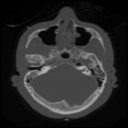
\includegraphics[width=1\linewidth]{images/VisMale_slice.jpg}
%		\caption{A sliced image of the data set}
%		\label{fig:VisMale_slice}
%	\end{minipage}~
%	\begin{minipage}{0.25\textwidth}
%		\centering
%		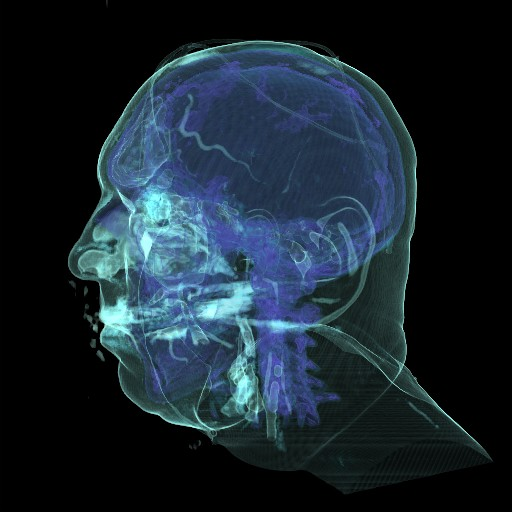
\includegraphics[width=1\linewidth]{images/VisMale.jpg}
%		\caption{Volume rendering of the data set}
%		\label{fig:VisMale}
%	\end{minipage}
%	\caption{The VisMale data set \cite{website:Roettger_volume_2013}}
%	\label{fig:multiple_VisMale}
%\end{figure}

\begin{figure}
\centering
\begin{minipage}{.25\textwidth}
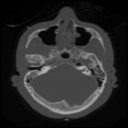
\includegraphics[width=1\linewidth]{images/VisMale_slice.jpg}
\caption{A sliced image of the data set}
\label{fig:VisMale_slice}
\end{minipage}~
\begin{minipage}{.25\textwidth}
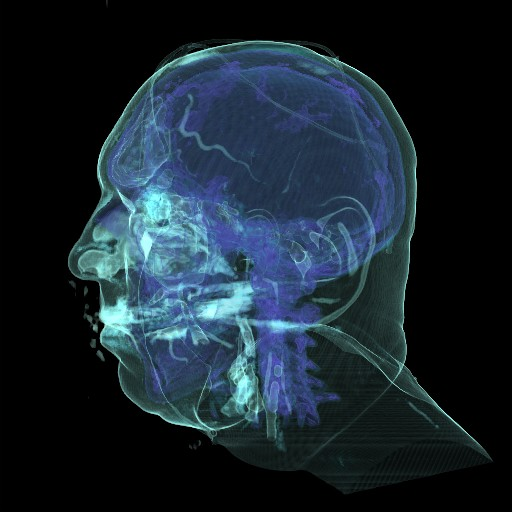
\includegraphics[width=1\linewidth]{images/VisMale.jpg}
\caption{Volume rendering of the data set}
\label{fig:VisMale}
\end{minipage}
\caption{The VisMale data set \cite{website:Roettger_volume_2013}}
\label{fig:multiple_VisMale}
\end{figure}

%Whereas rendering from polygonal representations extracted from volumetric datasets is also called indirect volume rendering.

%There are four typical volume rendering techniques: ray casting, splatting, shear warp and texture mapping. In recent years, many variants and combinations of these techniques have been proposed, especially approaches which utilise GPU hardware to improve performance or even achieve real-time interactivity.

%A volume renderer maps every voxel (an element in volume data) to an opacity and a colour with a transfer function, which is a piecewise linear function or an arbitrary table. Once converted to an RGBA value, the composed RGBA result is projected on corresponding pixel of the frame buffer with certain volume rendering techniques.

\section{Transfer Functions \label{literature_of_transfer_function}}
Volume data are 3D entities with information inside them, but the data might not consist of surfaces and edges.
%, or might be too voluminous to be represented geometrically.
%The goal of volume visualization is to gain insightful depictions of volume data.
Because of the lack of explicit geometric information, %and limited semantics, 
it is a major challenge to provide clear visualizations of the structures contained in a volume dataset.
Volume data may be rendered directly by mapping scalar values to visual properties (e.g. opacity and colour), or an intermediate geometric representation may be extracted using techniques like Marching Cubes \cite{lorensen_marching_1987} and then rendered as geometric surfaces. The mapping, which assigns visual properties to volume data, is called a transfer function.

Transfer function specification is an essential part in volume visualization.
%In terms of dimensionality, transfer functions are divided into two categories, one-dimensional (1D) and multidimensional.
A simple one-dimensional transfer function is a mapping from scalar values to RGB and alpha values.
The resulting visualization largely depends on how well the transfer function captures features of interest \cite{kniss_multidimensional_2002}.
%Due to the complex nature of volumetric datasets, abstraction techniques is often used in order to provide better understanding of the datasets.
However, it is non-trivial to obtain an effective transfer function. The specification is often a trial-and-error process, which involves a significant amount of tweaking of colour and opacity. Figure~\ref{fig:multiple_glk_transfunction} shows how slight changes in the transfer function lead to significant changes in the resulting images. The adjustment of transfer functions is unintuitive and often difficult.

\begin{figure}
        \centering
        \begin{minipage}{0.5\textwidth}
                \centering
                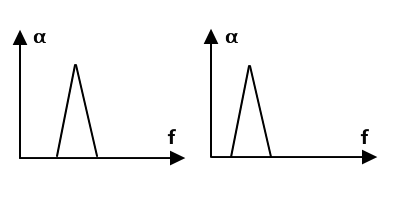
\includegraphics[width=1\linewidth]{images/glk_transfunction_tf.png}
                \caption{Two transfer functions (TF)}
                \label{fig:glk_transfunction_tf}
        \end{minipage}~
        \begin{minipage}{0.25\textwidth}
                \centering
                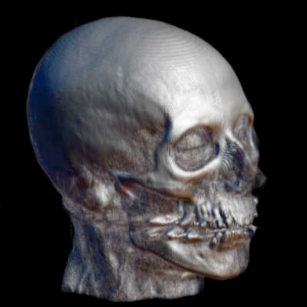
\includegraphics[width=1\linewidth]{images/glk_transfunction_1.png}
                \caption{The result from the TF on the left in \ref{fig:glk_transfunction_tf}}
                \label{fig:glk_transfunction_1}
        \end{minipage}~
        ~ %add desired spacing between images, e. g. ~, \quad, \qquad etc.
          %(or a blank line to force the subfigure onto a new line)        
        \begin{minipage}{0.25\textwidth}
                \centering
                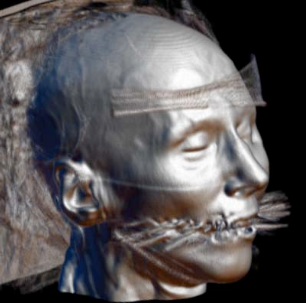
\includegraphics[width=1\linewidth]{images/glk_transfunction_2.png}
                \caption{The result from the TF on the right in \ref{fig:glk_transfunction_tf}}
                \label{fig:glk_transfunction_2}
        \end{minipage}    
        \caption{Slight changes in the transfer function causes significant difference in the resulting images \cite{kindlmann_transfer_2002}}
        \label{fig:multiple_glk_transfunction}
\end{figure}

In practice, major factors that have a great influence on transfer function setting are: partial volume effect \footnote{During the acquisition of data, the finite resolution causes contributions of different materials combined into the value of a single voxel. This is generally referred to as the partial volume effect, which results in blurred boundaries and hampers the detection of small or thin structures. \cite{serlie_classifying_2007}}, non-uniform distribution of materials and noise \cite{serlie_computed_2003}.
Among these, two challenging problems that need to be tackled could be elaborated as follows: firstly, for volume datasets, e.g. those obtained by MRI and CT, different tissues are represented in similar or even overlapping ranges of scalar values; secondly, interesting interior structures are often partly or completely occluded by surrounding tissue.
%This is common in visualizing interior structures. 
Consequently, feature detection and understanding volume data become a big challenge.

In volume rendering, these problems are handled by transfer function specification.
Good transfer functions reveal important structures in the data without obscuring them with less important regions.
%Traditional one-dimensional transfer function approaches, which assign optical properties only based on scalar value, are inadequate to extract inner structures of interest from volume data.
Various strategies have been proposed to simplify transfer function specification \cite{pfister_transfer_2001}.
Data-centric strategies examine the properties of volume data sets. Overlapping intensity intervals corresponding to different materials make boundary detection difficult. Classical approaches try to detect boundary information between tissues by introducing derived attributes such as first and second-order derivatives to isolate materials \cite{kindlmann_semi-automatic_1998} \cite{kniss_multidimensional_2002}. In this case, the transfer functions are extended to multidimensional feature spaces. As a result, the interaction of transfer functions becomes more complex and unintuitive.
There are other multi-dimensional transfer functions approaches, such as spatialized gradient-based transfer functions \cite{roettger_spatialized_2005}, distance-based transfer functions \cite{tappenbeck_distance-based_2006}, size-based transfer function \cite{correa_size-based_2008}, texture-based transfer functions \cite{caban_texture-based_2008} and curvature based transfer functions \cite{kindlmann_curvature-based_2003}.
Another strategy is based on the selection of rendered images. This strategy lets the user select one or more favourite images to guide the further search of transfer functions \cite{marks_design_1997} \cite{wu_interactive_2007}. More recent approaches introduced visibility \cite{correa_visibility_2011} or measures derived from information theory \cite{haidacher_information-based_2008} \cite{bruckner_isosurface_2010} \cite{ruiz_automatic_2011} \cite{bramon_information_2013}. Despite the advances of these methods, transfer function design for volume rendering is still an open research problem.

However, certain features of interest in volume data are difficult to extract and visualize with 1D transfer functions. For instance, many medical data sets created from CT or MRI scans contain a complex combination of boundaries between multiple materials. This situation is problematic for 1D transfer functions because of the potential for overlap between the data value intervals spanned by the different boundaries. When one data value or data range is associated with multiple boundaries, a 1D transfer function is unable to render them in isolation \cite{kniss_multidimensional_2002}.

The introduction of multidimensional transfer functions alleviates this problem.
Instead of classifying a sample based on a single scalar value, multi-dimensional transfer functions allow a sample to be classified based on a combination of values.
Multidimensional transfer functions are very effective means to extract materials and their boundaries for both scalar and multivariate data. However, the parameter spaces of multidimensional transfer functions are more complex (compared to 1D transfer functions) and thus introduce problems such as requirement for large amount of user interaction, missing precision or the means of handling it being unintuitive \cite{arens_survey_2010}.

Moreover, transfer function specification in general is an unintuitive or even monotonous task for average users, because it is usually an iterative process of trial and error.
For instance, there are skin and fat tissues around the brain, and their intensities lie in the same range as the brain. If we want to visualize the brain by setting the scalar value range of the brain to opaque, the surrounding skin and fat tissue will also become opaque. Then the brain will be occluded by the surrounding soft tissues which make it difficult to explore the brain structure.
Common approaches to this problem are to introduce explicit segmentation of structures of interest before the volume rendering process \cite{rezk-salama_opacity_2006}. In fact, the process of applying the transfer function could be interpreted as a segmentation problem.

\subsection{Multidimensional Transfer Functions}
Multidimensional transfer functions \cite{kindlmann_semi-automatic_1998} \cite{kniss_interactive_2001} \cite{kniss_multidimensional_2002}, which are mappings from intensity and other variables, such as first and second derivatives to colour and opacity, have demonstrated their effectiveness in distinguishing boundaries between materials in volume data. For higher-dimensional transfer functions, the generation of transfer functions could be memory intensive and costly to compute, and exploration of the transfer function domain might not be intuitive.
Therefore, two-dimensional (2D) histograms are often used in multidimensional transfer functions \cite{maciejewski_structuring_2009}. An example is a 2D histogram with axes representing a subset of the feature space (e.g. scalar value vs gradient magnitude), with each entry in the 2D histogram being the number of voxels for a given feature space pair.
%A great number of transfer function approaches have also been merged and one-dimensional transfer function is extended to multi-dimensional transfer function.

As one of the most common representations of voxel distributions, histograms are used in transfer function design to assign visual properties to voxels \cite{pfister_transfer_2001}. Bajaj et al. \cite{bajaj_contour_1997} introduced the contour spectrum to determine voxels corresponding to important isosurfaces in the volume. To overcome the difficulty of using one-dimensional transfer functions (solely based on scalar values stored in the voxels) to extract inner structures of interest from the volume data, Levoy proposed the use of gradient magnitude to emphasize strong boundaries between different tissues \cite{levoy_display_1988}.

The introduction of gradient magnitude as a data metric aims to detect voxels that are of large deviation compared with other voxels by approximating gradient magnitude at each sample point in the volume, because the exact distribution of data is unknown due to information lost in the discrete sampling process.

Kindlmann and Durkin extended Levoy's work by introducing a higher dimensional transfer function domain based on gradient magnitudes and second derivatives \cite{kindlmann_semi-automatic_1998}. To emphasize different structures, Kniss et al. \cite{kniss_interactive_2001} presented a technique for interactively manipulating 2D histograms of gradient magnitudes and data values. In their work, material boundaries appear as arcs in the 2D histogram and can be selected with interactive widgets \cite{kniss_multidimensional_2002}.
Kindlmann et al. \cite{kindlmann_curvature-based_2003} proposed curvature-based transfer function to enhance the expressive and informative power of volume rendering. In their approach, volume data is rendered with contours to exhibit constant thickness in image space.
Maciejewski et al. proposed a non-parametric method to generate transfer function \cite{maciejewski_structuring_2009}. Wang et al. introduced clustering of 2D density plots in their automating transfer function \cite{wang_automating_2012}.

\cite{ip_hierarchical_2012}
\cite{maciejewski_abstracting_2013}
\cite{fang_visualization_2007}
\cite{akiba_simultaneous_2006}
%\paragraph{Isosurface Statistics}
%Geometric properties of isosurfaces
%\cite{bruckner_isosurface_2010}

%\paragraph{Clustering}

\subsection{Transfer Functions for Time-Varying Volume Visualization}
Although researchers have developed a great number of visualization techniques for time-invariant volume data, how to effectively explore and understand time-varying volume data remains a challenging problem. Finding good transfer functions for time-invariant volume data itself has proven difficult \cite{pfister_transfer_2001}.
%Finding good transfer functions for time-varying volume data is even more difficult, as data value ranges and distributions change over time.
%Although researchers have developed a great number of visualization techniques for static volume data, how to effectively explore and understand time-varying volume data remains a challenging problem.
Finding good transfer functions for time-varying volume data is more difficult than for static volume data, as data value ranges and distributions change over time.

Coherence is an important issue of transfer function design for time-varying volume data. Ideally, a single transfer function should be used for the whole time-varying data set in order to obtain coherent visualization. More than one color or opacity map can be misleading or physically meaningless, because the transition from one transfer function to another may cause sudden changes in the resulting images. However, this practice is not always applicable to general time-varying data sets.

%Jankun-Kelly and Ma \cite{jankun-kelly_study_2001} examined how to combine transfer functions for different time-steps to generate a coherent transfer function.
Jankun-Kelly and Ma \cite{jankun-kelly_study_2001} examined how to combine transfer functions for different time-steps to generate a coherent transfer function.
Woodring et al. \cite{woodring_high_2003} considered time-varying volume data as four-dimensional data field and provided a user interface to specify hyperplanes in 4D.
Woodring and Shen \cite{woodring_chronovolumes_2003} introduced an alternative approach to render multiply time-steps in a sequence with different colours into a single image. This approach provides the context of surrounding time steps but coherence of colour among time-steps is hard to maintain.
%Tikhonova et al. \cite{tikhonova_exploratory_2010} presented an exploratory approach based on a compact representation of each time step of the dataset in the form of ray attenuation functions. Ray attenuation functions are subsequently used for transfer function generation.
Tikhonova et al. \cite{tikhonova_exploratory_2010} presented an exploratory approach based on a compact representation of each time step of the dataset in the form of ray attenuation functions. Ray attenuation functions are subsequently used for transfer function generation.

\section{Automated Transfer Function Optimization}
Various strategies have been proposed to simplify transfer function specification \cite{pfister_transfer_2001}.
%Data-centric strategies examine the properties of volume data sets.
Overlapping intensity intervals corresponding to different materials make boundary detection difficult. Classical approaches try to detect boundary information between tissues by introducing derived attributes such as first and second derivatives to isolate materials \cite{kindlmann_semi-automatic_1998} \cite{kniss_multidimensional_2002} \cite{kindlmann_transfer_2002}.
In this case, the transfer functions are extended to multidimensional feature spaces. As a result, the interaction of transfer functions becomes more complex and unintuitive as the dimensionality becomes higher.
%Even two-dimensional transfer functions require a considerable amount of user interaction to find a meaningful shape \cite{arens_survey_2010}.
Even in the case of two-dimensional transfer functions, a considerable amount of user interaction is
required in order to come up with meaningful results \cite{arens_survey_2010}.
%There are other multi-dimensional transfer functions approaches, such as spatialized gradient-based transfer functions \cite{roettger_spatialized_2005}, distance-based transfer functions \cite{tappenbeck_distance-based_2006}, size-based transfer function \cite{correa_size-based_2008}, texture-based transfer functions \cite{caban_texture-based_2008} and curvature based transfer functions \cite{kindlmann_curvature-based_2003}.

Rezk-Salama et al. \cite{rezk-salama_automatic_2000} presented high-level semantics to abstract parametric models of transfer functions in order to automatically assign transfer function templates.
Bruckner and Gr{\"o}ller introduced the concept of style transfer functions \cite{bruckner_style_2007}, which aim to produce more comprehensible images by using transfer functions that map input values to different non-photorealistic rendering styles.
%Another strategy is based on the selection of rendered images. This strategy lets the user select one or more favorite images to guide the further search of transfer functions
%\cite{marks_design_1997}.
Wu and Qu \cite{wu_interactive_2007} developed a method that uses editing operations and stochastic search of the transfer function parameters to maximize the similarity between volume-rendered images given by the user.


\section{chapter 4}
Transfer functions have played a crucial role in volume visualization and the design of transfer functions to generate informative visualizations has been a significant challenge addressed by a number of researchers \cite{pfister_transfer_2001}.
Various strategies have been proposed to simplify transfer function specification \cite{hadwiger_real-time_2006}.
In volume data, boundaries are regions between areas of relatively homogeneous material. It is difficult to detect boundaries because different materials often consist of overlapping intensity intervals. To address this problem, multidimensional transfer functions used derived attributes such as gradient magnitudes and second derivatives along with scalar values, in order to detect transitions between relatively homogeneous areas \cite{kindlmann_semi-automatic_1998} \cite{kniss_multidimensional_2002} \cite{kindlmann_transfer_2002}.
%Classical approaches try to detect boundary information between tissues by introducing derived attributes such as first and second derivatives to isolate materials \cite{kindlmann_semi-automatic_1998} \cite{kniss_multidimensional_2002} \cite{kindlmann_transfer_2002}.
In this case, the transfer functions are extended to multidimensional feature spaces. As a result, the interaction of transfer functions becomes more complex and unintuitive as the dimensionality becomes higher.
Even in the case of two-dimensional transfer functions, a considerable amount of user interaction is
required in order to come up with meaningful results \cite{arens_survey_2010}.

\section{Visibility Histograms}
\cite{emsenhuber_visibility_2008}

\cite{correa_visibility_2011}

\cite{wang_efficient_2011}

\section{Information Theory in Visualization}
Information theory \cite{shannon_mathematical_1948} was originally introduced to study the fundamental limit of reliable transmission of messages through a noisy communication channel. Traditional applications of information theory, such as data compression and data communication, focus on the efficient throughput of a communication channel, whilst visualization focuses on the effectiveness in aiding the perceptual and cognitive process for data understanding and knowledge discovery.

In recent years, there is an emerging direction towards using the principles of information theory to solve challenging problems in scientific visualization. \cite{wang_information_2011}. Chen and J�enicke \cite{chen_information-theoretic_2010} presented an information-theoretic framework for visualization. They examined the theoretical aspect of information and its relation to data communication and interpret different stages of the visualization pipeline using the taxonomy of information.

Haidacher et at. \cite{haidacher_information-based_2008} proposed an approach of transfer function specification for multi-modal data visualization. They considered the joint occurrence of multiple features from one or multiple variables so as to separate statistical features that only occur in a single variable from those that are present in both.
Ruiz et al. \cite{ruiz_automatic_2011} presented an approach to generate transfer functions from a target distribution provided by the user. Their approach is based on a communication channel between a set of viewpoints and a set of bins of a volume data set, and supports both 1D and 2D transfer functions including the gradient information.
Bramon et al. \cite{bramon_information_2013} proposed an automatic method to visualize multi-modal data by combining several information-theoretic strategies to define colours and opacities of the multi-modal transfer function.
They set an information channel between two registered input datasets to define the fused colour and minimize the informational divergence between the visibility distribution captured by a set of viewpoints and a target distribution proposed by the user to obtain the opacity.

\section{Saliency}
\cite{itti_model_1998}

\cite{harel_graph-based_2006}

\cite{cui_measuring_2006}

\cite{lee_mesh_2005}

\cite{duan_visual_2011}

\cite{kim_saliency-guided_2006}

\cite{shen_spatiotemporal_2015}

\section{Non-Photorealistic Rendering (NPR)}
In contrast to traditional computer graphics, which has focused largely on creating photorealistic images of synthetic objects, non-photorealistic rendering (NPR) is an area of computer graphics that focuses on creating abstract images with a wide variety of expressive styles \cite{haeberli_paint_1990}. NPR has been an active research area for a long time. A number of approaches have been proposed to produce convincing artistic styles for both off-line and on-line rendering. For example, there are various types of commonly used styles including painterly rendering, edge stylisation, sketch-shading, cel-shading, hatching.
% Although there are plenty of works on non-photorealistic rendering, most of them focus on how to imitate artistic styles with emphasis on aesthetic aspects.
%Researchers in modelling and rendering in computer graphics have focused for many years on producing photorealistic images, which are indistinguishable from photographs captured from real-world scene. Nevertheless, there are other compelling methods of visual discourse such as paintings, sketches and cel animation.
In certain situations, non-photorealistic renderings are considered more effective and expressive than an equivalent photograph \cite{healey_perceptually_2004}.

%As a basic part of most approaches to non-photorealistic volume rendering, contours delineate object shape and clarify sites of occlusion by emphasizing the transition between front-face and back-facing surface locations.
%Kindlmann et al. \cite{kindlmann_curvature-based_2003} proposed curvature-based transfer function to enhance the expressive and informative power of volume rendering. In their approach, volume data is rendered with contours to exhibit constant thickness in image space.

\subsection{Illustrative Visualization}
NPR models were adopted in visualization and hence formed the field illustrative visualization.
Illustrative visualization, as a novel category of visualization, aims at visualizing data in a clear and understandable way using techniques from traditional hand-crafted illustrations. Illustrative visualization has been successful employed in medical visualization \cite{svakhine_illustration_2005} \cite{viola_importance-driven_2005}.
Illustration-based styles are believed to be effective in conveying information. Researchers in the field of computer graphics and visualization have applied illustration-based styles in order to produce effective and expressive visualization. Stompel et al. \cite{stompel_visualization_2002} introduced feature enhancement techniques, such as strokes based, temporal domain enhancement, to enhance time-varying data obtained from the field of computational fluid dynamics (CFD).

\subsection{Visualising Time-Varying Volume Data with NPR}
An essential problem in time-varying volume visualization is to visualize temporal variation and analysis of features. Traditionally, time-varying data has been visualized as snapshots of individual time steps or animation of snapshots of a sequence of time steps. These techniques are effective in making time-varying data understandable. However, they struggle when the complexity of datasets increased dramatically in recent years \cite{brambilla_illustrative_2012}.

Compared to flow visualization, which is a well established branch of scientific visualization \cite{brambilla_illustrative_2012}, general time-varying volume visualization is still a relative young field.
Illustrations for time-varying rendering could be divided into two categories, one is to enhance time-invariant features and the other is to enhance temporal features of time-varying volume data. The techniques in the first category focus on enhancing structural perception of volume models through the amplification of features and the addition of illumination effects \cite{rheingans_volume_2001} \cite{joshi_illustration-inspired_2005}. Examples of these techniques include boundary enhancement, oriented feature enhancement (silhouettes, fading, and sketch lines). The techniques in the second category focus on illustrating dynamic aspects such as movement of features. A few kinds of techniques have been proposed for this purpose. For example, there are speadlines, flow ribbons and strobe silhouettes, which are inspired by traditional animation \cite{joshi_illustration-inspired_2005} \cite{joshi_evaluation_2008} \cite{joshi_case_2009}; and there are extended silhouette and boundary enhancement domains, which are inspired by the techniques used by illustrators and other artists \cite{svakhine_illustration_2005}. Nevertheless, illustrations of temporal features of time-varying data requires more attention from researchers in the visualization community. The usefulness of illustrative approaches in time-varying volume visualization has not been studied as thoroughly as in other areas.

\subsection{Painterly Stylization and Texture-Based Techniques \label{painterly_rendering}}
Streamlines and textures are often used to represent flow directions \cite{urnessy_techniques_2004}. Interrante and Grosch \cite{interrante_strategies_1997} introduced volume LIC (Line Integral Convolution) to visualize 3D flow via volume textures. Figure~\ref{fig:interrante_strategies_1997} shows a volume texture generated with LIC. In this figure, vorticity magnitude is mapped to streamline colour and the striations along the axial direction reveal the presence of periodic waves propagated down the jet axis. Since volume LIC is limited to steady flows, Liu and Moorhead \cite{liu_texture-based_2005} introduced a accelerated unsteady flow LIC algorithm to generate volume flow textures (Figure~\ref{fig:liu_texture-based_2005}). In their approach, magnitude-based transfer functions and cutting planes in volume rendering are employed to show the flow structure and the flow evolution.

Artists recognize patterns and flows in a target scene and express them through brush strokes. They use stroke orientation corresponding to the actual movement \cite{lee_motion_2009}. This type of techniques from master painting and human perception are used to visualize multidimensional data sets \cite{healey_perceptually_2004}. Tateosian et al. \cite{tateosian_engaging_2007} use the colour, orientation and size of strokes to represent the magnitude, flow orientation and pressure of a 2D slice of a simulated supernova collapse (Figure~\ref{fig:tateosian_engaging_2007}). Lee et at. \cite{lee_motion_2009} presented a painterly rendering technique based on the motion information (magnitude, direction, standard deviation) extracted from a image sequences of the same view.

\begin{figure}
\centering
\begin{minipage}{.49\textwidth}
  \centering
    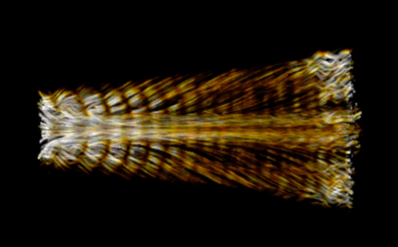
\includegraphics[width=1\linewidth]{images/interrante_strategies_1997.png}
  \caption{Streamlines are represented as a volume texture, which provides an intuitive impression of the 3D flow. \cite{interrante_strategies_1997}}
  \label{fig:interrante_strategies_1997}
\end{minipage}~
\begin{minipage}{.49\textwidth}
  \centering
    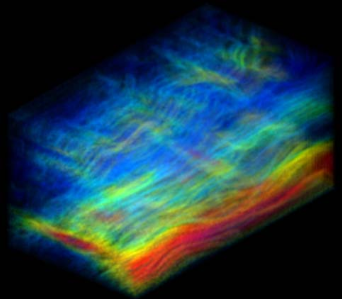
\includegraphics[width=1\linewidth]{images/liu_texture-based_2005.png}
  \caption{Streamlines are represented as a volume texture, which provides an intuitive impression of the 3D flow. \cite{liu_texture-based_2005}}
  \label{fig:liu_texture-based_2005}
\end{minipage}
\end{figure}

\begin{figure}
\centering
\begin{minipage}{.49\textwidth}
  \centering
    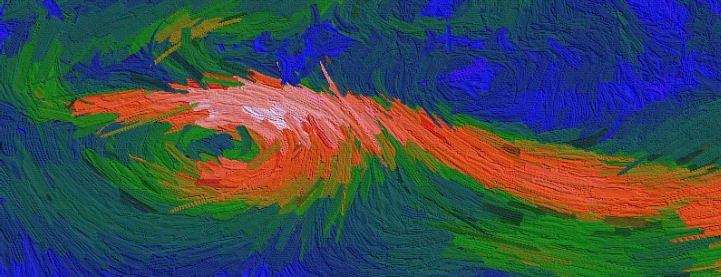
\includegraphics[width=1\linewidth]{images/tateosian_engaging_2007.png}
  \caption{A visual complexity style visualization of flow patterns in a 2D slice though a simulated supernova collapse, using the mappings: flow orientation $ \rightarrow $ stroke orientation, magnitude $ \rightarrow $ order and pressure $ \rightarrow $ stroke size \cite{tateosian_engaging_2007}.}
  \label{fig:tateosian_engaging_2007}
\end{minipage}~
\begin{minipage}{.49\textwidth}
  \centering
    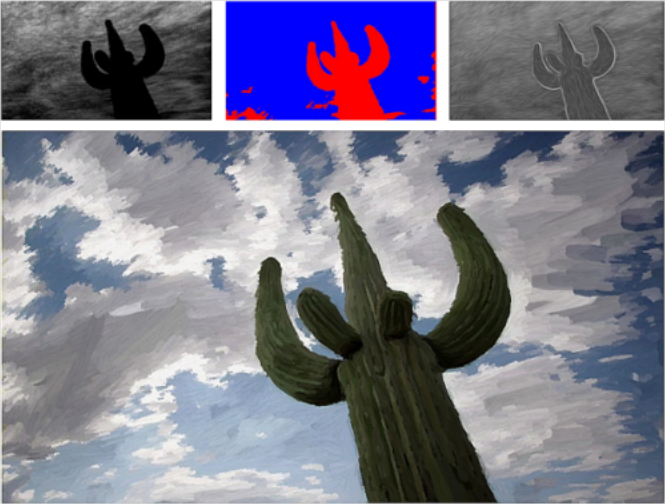
\includegraphics[width=1\linewidth]{images/lee_motion_2009.png}
  \caption{The motion directions determine stroke orientations in the regions with significant motions, and image gradients determine stroke orientations where little motion is observed \cite{lee_motion_2009}.}
  \label{fig:lee_motion_2009}
\end{minipage}
\end{figure}

\section{Feature Tracking}
Feature extraction and tracking is an established technique for the analysis of time-varying data in various research fields, such as video analysis, computer vision and flow visualization \cite{muelder_interactive_2009}.
In time-varying data, features are objects that evolve over time. Feature tracking aims to determine the correspondence between features in successive time steps and describe the evolution of features through time \cite{post_state_2003}.

In practice feature extraction and tracking are often employed in the exploration and analysis of time-varying volume visualization in order to better understand the dynamic nature of the underlying phenomena \cite{tzeng_intelligent_2005} \cite{woodring_multiscale_2009} \cite{lee_visualizing_2009} \cite{gu_transgraph_2011}.
Feature extraction methods are often based on an analytical description of the feature of interest. Consequently, feature extraction and tracking could become a manual-driven and trial-and-error process in the case that the properties cannot be easily defined and are sometimes unknown \cite{ma_machine_2007}.

%%survey
% \cite{ma_machine_2007} \cite{wang_information_2008}
%
%\cite{caban_texture-based_2007}
%
%%tracking related works
%\cite{widanagamaachchi_interactive_2012} \cite{ozer_group_2012}

\section{Vector Field Visualization}
The visualization of vector fields plays a crucial role in visual interpretation and understand of the underlying flow features and patterns \cite{kuhn_clustering-based_2011} \cite{ma_coherent_2013}. Since flow patterns also exist in time-varying volume data, certain techniques for visualizing vector field could be incorporated into time-varying volume visualization, in order to depict the dynamic aspects of time-varying data.

Line drawings are effective ways to depict complex information with simple means \cite{benard_state_art_2011}. Among vector field visualization techniques, streamline visualization is a simple but common way to convey the structure of 3D vector fields \cite{chen_illustrative_2011}. Streamlines have proven to give expressive visual representation if they are combined with appropriate seeding strategies \cite{annen_vector_2008}. Streamlines reveal flow patterns in an intuitive fashion by integrating the flow path.

\section{Perceptual Evaluation}
%The term visualization may have various meanings.
%Chen et al. \cite{chen_what_2013} presented a definition, which is "visualization is a study of transformation from data to visual representations in order to facilitate effective and efficient cognitive processes in performing tasks involving data". Therefore, based on this definition, the fundamental measure for effectiveness is correctness and that for efficiency is the time required for accomplishing a task.

Due to the complex nature of the data being studied, simply displaying all available information does not adequately meet the demands of domain scientists \cite{anderson_evaluating_2012}.
%Determining the best use of visualization techniques is one of the goals of visualization evaluations.
User studies can be used to evaluate the strengths and weaknesses of visualization methods \cite{christopher_thoughts_2003}.
The evaluation of visualization methods that focus on human factors often employ user studies or expert evaluations to determine their effects on interpretation and usability.

There are a number of different evaluation strategies, such as measuring user performance, accuracy and experience \cite{redmond_influencing_2010}. Laidlaw et al. \cite{laidlaw_quantitative_2001} compared six methods for visualising 2D vector fields and measured user performance on three flow-related tasks for each of the six methods. They used the evaluation results to identify what makes a 2D vector fields visualization effective.
Joshi and Rheingans \cite{joshi_evaluation_2008} evaluated the effective of their illustrative techniques by measuring user accuracy, time required to perform a task and user confidence.

\section{Summary}
We have presented a review of the literature in the field of volume visualization.
The review suggests that it is feasible to optimise the parameters of volume visualization based on the information within the volume data. Existing research on multidimensional transfer functions, classification of volume data and information theory provides us the foundation to explore and understand how this optimisation may be achieved.
%Existing research on the analysis and visualization of time-varying data and flow data gives us valuable information on the study of the dynamic aspect of time-varying volume data.
In particular, the analysis and visualization of time-varying data is a compelling problem due to increasing availability of such data in recent years. Although some work has been published in this area it is clear that there is compelling work left to be done in optimising the rendering of such data sets.
The use of NPR techniques can improve the expressiveness of the visualization and thus facilitate better user understanding of data.
Further studies are required in order to better integrate NPR techniques into the visualization pipeline and enhance the expressiveness of the visualization by exploiting the information within the data sets.

%-------------------------------------------------------------------------
